\documentclass[conference]{IEEEtran}
\IEEEoverridecommandlockouts
% The preceding line is only needed to identify funding in the first footnote. If that is unneeded, please comment it out.
\usepackage{cite}
\usepackage{amsmath,amssymb,amsfonts}
\usepackage{algorithmic}
\usepackage{graphicx}
\usepackage{textcomp}
\usepackage{xcolor}
\def\BibTeX{{\rm B\kern-.05em{\sc i\kern-.025em b}\kern-.08em
    T\kern-.1667em\lower.7ex\hbox{E}\kern-.125emX}}
\begin{document}

\title{Summer School Summary-Fang Qing}

\author{Qing Fang}

\maketitle

\begin{abstract}
    During the summer school, I chose the ICN direction, 
    read related books ("Information Center Network and Named Data Network") and papers, 
    and reported twice a week. 
    At the same time, the configuration of the minindn experimental environment was carried out, 
    and the processing of the Interest packet in the NFD forwarding process 
    and the related function calls and logical relations were learned. 
    At the same time, I taught myself the related operations of git and latex. All in all, I learned a lot.
\end{abstract}


\section{Information Center Network and Named Data Network}
After reading the first to eighth chapters of the book "Information Center Network and Named Data Network", I have to say that this book is a good learning material for a beginner in ICN.


First, through the study of this book, I understand the necessity of the birth of ICN. Due to the exposure of various "problems" in IP networks, the emergence of ICN undoubtedly provides new ideas for solving problems.


Second, through reading, I understand the design ideas and architecture of the NDN architecture, including NDN naming, security mechanisms, routing and forwarding, caching, and transmission.


Because the NDN network is name-centric, because the naming mechanism is very important. In the process of naming mechanism, it mainly describes the hierarchical naming method, naming attributes and principles, and gives examples.


And compared NDN with other ICN networks, focusing on comparing NDN with TCP/IP, which more clearly reflects the advantages of NDN.


\subsection{NDN architecture}

\begin{figure}[htbp]
    \centerline{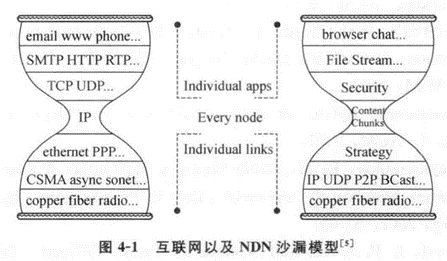
\includegraphics{NDN architecture.png}}
    \caption{NDN architecture}
    \label{fig}
\end{figure}
There are two more layers in NDN: policy layer and security layer.

\begin{figure}[htbp]
    \centerline{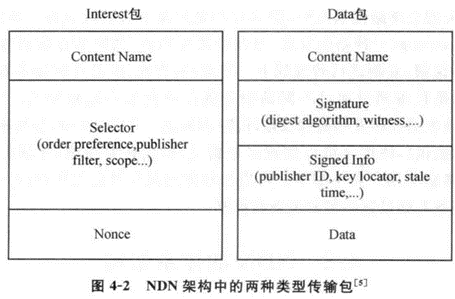
\includegraphics{packet.png}}
    \caption{NDN architecture}
    \label{fig}
\end{figure}

As the unique identifier of the package, the Content Name is equivalent to the ip address in the ip protocol.
NDN uses an in-network caching mechanism, and FIB is used to route request packets to potential matching data sources, using the longest match <prefix, interface list>. The PIT saves the upstream information of the Interest packet to ensure that if the current node has trusted data, it can easily send the data to the receiver in the opposite path.


The name structure of NDN is shown in the figure below.
\begin{figure}[htbp]
    \centerline{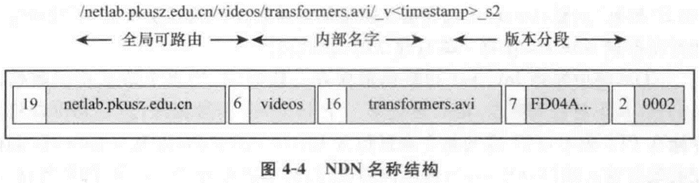
\includegraphics{NDN name architecture.png}}
    \caption{NDN name architecture}
    \label{fig}
\end{figure}


\subsection{NDN's caching mechanism}
As mentioned in the book, one of the principles of NDN network design is to deploy network caches as large as possible, maximize bandwidth usage, and achieve fast, reliable, and scalable content delivery to avoid congestion. In-Network Cache is adopted: routing nodes on the transmission path can cache objects passing through it (one of the important characteristics of NDN distinguishing IP networks). The caching strategies adopted are: Least Recently Used (LRU) and Least Frequently Used (LFU). Of course, there are other strategies, so I won't elaborate on them one by one here. Finally, a comparison of the advantages and disadvantages of common caching strategies is made.


\subsection{NDN routing and forwarding}
\subsubsection{routing}
The traditional IP network uses the OSPF protocol, OSPF, open shortest path first. It proves that the link state routing protocol can better support multi-path routing and converge at a faster speed, so NDN chooses to extend OSPF to implement the first name-based routing protocol, OSPFN (OSPF for NDN). OSPFN uses OLSA to advertise the prefix of the name, allowing applications to specify the information that needs to be broadcast on the network. However, because OSPFN does not support dynamic multi-path forwarding and does not establish a mechanism to authenticate routing data, NLSR came into being. NLSR is called named data link state routing protocol. NLSR uses names to identify routers and links, and routers use the signature of each routing information to verify its original source and authenticity.

\subsubsection{forwarding}
\begin{figure}[htbp]
    \centerline{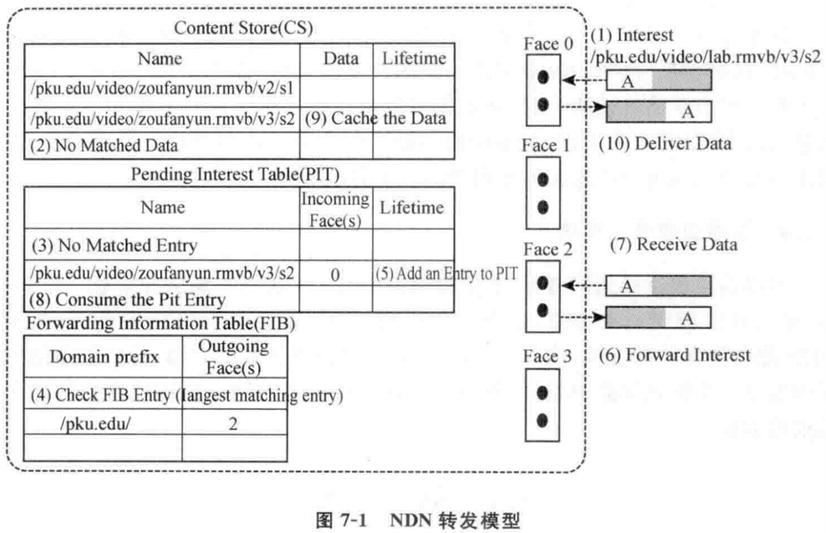
\includegraphics{forwarding model.png}}
    \caption{forwarding model}
    \label{fig}
\end{figure}
The forwarding model is shown in the figure. NDN is also called smart forwarding, compared to smart routing and clumsy forwarding in IP networks. Because the NDN forwarding process will be controlled by factors such as state mechanisms, interface sequencing, rate limiting, and congestion control, so as to ensure reasonable forwarding.


\section{Paper Reading}

During the summer study, the brother gave several basic papers and several research papers. 
After reading several papers, I have a better understanding of ICN and NDN.


Through the learning of ICN path switching, I understand how ICN discovers 
and guides paths during data transmission. There is a crucial thing called "path tags". 
And the forwarding plane after the introduction of the path label is 
compared with the previous forwarding process. After experimental evaluation, 
it is found that after the introduction of the path label, the forwarding will not be affected, 
and it can also show a good response to the routing update, and has good forwarding scalability.


Next, an assessment was made on the application of NDN network in real-time traffic. 
Nowadays, the requirements for real-time video QoS are getting higher and higher, 
and real-time video traffic is gradually increasing, so such a design is proposed. 
Finally, NLB, Ucast, and Bcast are evaluated in terms of scalability of the number of clients, 
packet redundancy, and CPU usage. Experiments show that NLB shows good results in these three aspects.


Finally, I read a paper entitled "A Practical Congestion Control Scheme for Named Data Networks", 
and proposed a practical congestion control scheme PCON to solve the NDN architecture. 
The congestion control scheme must consider intra-network caching and multi-path forwarding. 
And the impact of multicast data delivery. PCON detects congestion based on 
CoDel AQM (by measuring message queuing time), and sends congestion signals to 
consumers by explicitly marking specific messages, so that downstream routers 
can transfer traffic to other paths, and consumers can reduce Interest sending rate. 
Finally, the same experimental simulation shows that PCON's forwarding adaptation 
has achieved a higher total throughput than the existing work, while maintaining similar RTT fairness. 
In addition, PCON can adapt to changes in IP tunnel and wireless link capacity, which is a condition 
that other hop-by-hop solutions cannot consider.

\section{Others}
Regarding the study of other content, I have recorded it and wrote several blogs, please refer to:


1. Configuration of minindn environment:


https://www.cnblogs.com/laysfq/p/15229289.html




2. The NFD forwarding process processes the Interest packet:


https://www.cnblogs.com/laysfq/p/15273038.html




3. Various git operations: basic operations and multi-person collaboration and conflict resolution:


https://www.cnblogs.com/laysfq/p/15273002.html

\section{Conclusion}
Although the summer school only lasted more than a dozen days, it gave me a preliminary understanding of ICN and NDN, and I have become interested in them. The several papers I read during the summer study made me feel that there is still a lot of research space for NDN in terms of congestion control and forwarding strategies, but I gradually discovered that there is still a lot of content about NDN in the process of constantly searching papers. For example, a paper I was reading recently "f-NDN: An Extended Architecture of NDN Supporting Flow Transmission Mode", the NDN extended architecture that supports the streaming transmission mode is to perform stream processing on a single data during the forwarding process. Thereby improving efficiency.


This also reflects that for me at the moment, I need to read a lot of papers and accumulate basic knowledge. Only when I have enough depth and breadth of the subject can I produce my own idea.


I hope that after three years, I can have a share of my own in the research field of NDN, so keep going!

\end{document}
